%%%%%%%%%%%%%%%%%%%%%%%%%%%%%%%%%%%%%%%%%
% Journal Article
% Database System
% Practical 7: Implementation of sorting based two pass algorithm
%
% Gahan M. Saraiya
% 18MCEC10
%
%%%%%%%%%%%%%%%%%%%%%%%%%%%%%%%%%%%%%%%%%
%----------------------------------------------------------------------------------------
%       PACKAGES AND OTHER DOCUMENT CONFIGURATIONS
%----------------------------------------------------------------------------------------
\documentclass[paper=letter, fontsize=12pt]{article}
\usepackage[english]{babel} % English language/hyphenation
\usepackage{amsmath,amsfonts,amsthm} % Math packages
\usepackage[utf8]{inputenc}
\usepackage{xcolor}
\usepackage{float}
\usepackage{lipsum} % Package to generate dummy text throughout this template
\usepackage{blindtext}
\usepackage{graphicx} 
\usepackage{caption}
\usepackage{subcaption}
\usepackage[sc]{mathpazo} % Use the Palatino font
\usepackage[T1]{fontenc} % Use 8-bit encoding that has 256 glyphs
\usepackage{bbding}  % to use custom itemize font
\linespread{1.05} % Line spacing - Palatino needs more space between lines
\usepackage{microtype} % Slightly tweak font spacing for aesthetics
\usepackage[hmarginratio=1:1,top=32mm,columnsep=20pt]{geometry} % Document margins
\usepackage{multicol} % Used for the two-column layout of the document
%\usepackage[hang, small,labelfont=bf,up,textfont=it,up]{caption} % Custom captions under/above floats in tables or figures
\usepackage{booktabs} % Horizontal rules in tables
\usepackage{float} % Required for tables and figures in the multi-column environment - they need to be placed in specific locations with the [H] (e.g. \begin{table}[H])
\usepackage{hyperref} % For hyperlinks in the PDF
\usepackage{lettrine} % The lettrine is the first enlarged letter at the beginning of the text
\usepackage{paralist} % Used for the compactitem environment which makes bullet points with less space between them
\usepackage{abstract} % Allows abstract customization
\renewcommand{\abstractnamefont}{\normalfont\bfseries} % Set the "Abstract" text to bold
\renewcommand{\abstracttextfont}{\normalfont\small\itshape} % Set the abstract itself to small italic text
\usepackage{titlesec} % Allows customization of titles

\renewcommand\thesection{\Roman{section}} % Roman numerals for the sections
\renewcommand\thesubsection{\Roman{subsection}} % Roman numerals for subsections

\titleformat{\section}[block]{\large\scshape\centering}{\thesection.}{1em}{} % Change the look of the section titles
\titleformat{\subsection}[block]{\large}{\thesubsection.}{1em}{} % Change the look of the section titles
\newcommand{\horrule}[1]{\rule{\linewidth}{#1}} % Create horizontal rule command with 1 argument of height
\usepackage{fancyhdr} % Headers and footers
\pagestyle{fancy} % All pages have headers and footers
\fancyhead{} % Blank out the default header
\fancyfoot{} % Blank out the default footer

\fancyhead[C]{Institute of Technology, Nirma University $\bullet$ October 2018} % Custom header text

\fancyfoot[RO,LE]{\thepage} % Custom footer text
%----------------------------------------------------------------------------------------
%       TITLE SECTION
%----------------------------------------------------------------------------------------
\title{\vspace{-15mm}\fontsize{24pt}{10pt}\selectfont\textbf{Practical 7: Implementation of sorting based two pass algorithm}} % Article title
\author{
\large
{\textsc{Gahan Saraiya, 18MCEC10 }}\\[2mm]
%\thanks{A thank you or further information}\\ % Your name
\normalsize \href{mailto:18mcec10@nirmauni.ac.in}{18mcec10@nirmauni.ac.in}\\[2mm] % Your email address
}
\date{}
\hypersetup{
	colorlinks=true,
	linkcolor=blue,
	filecolor=magenta,      
	urlcolor=cyan,
	pdfauthor={Gahan Saraiya},
	pdfcreator={Gahan Saraiya},
	pdfproducer={Gahan Saraiya},
}
%----------------------------------------------------------------------------------------
\usepackage[utf8]{inputenc}
\usepackage[english]{babel}
\usepackage[utf8]{inputenc}
\usepackage{fourier} 
\usepackage{array}
\usepackage{makecell}

\renewcommand\theadalign{bc}
\renewcommand\theadfont{\bfseries}
\renewcommand\theadgape{\Gape[4pt]}
\renewcommand\cellgape{\Gape[4pt]}
\newcommand*\tick{\item[\Checkmark]}
\newcommand*\arrow{\item[$\Rightarrow$]}
\newcommand*\fail{\item[\XSolidBrush]}
\usepackage{minted} % for highlighting code sytax
\definecolor{LightGray}{gray}{0.9}

\setminted[text]{
	frame=lines, 
	breaklines,
	baselinestretch=1.2,
	bgcolor=LightGray,
%	fontsize=\small
}

\setminted[python]{
	frame=lines, 
	breaklines, 
	linenos,
	baselinestretch=1.2,
%	bgcolor=LightGray,
%	fontsize=\small
}

\begin{document}
\maketitle % Insert title
\thispagestyle{fancy} % All pages have headers and footers


\section{Introduction}
\paragraph{} Aim of this practical is to implement sort based two pass algorithm to find distinct values.

\section{Logic}
\paragraph{Prerequisite setup:} Created a data file and added dummy in it
\subsection{Pass 1}
	\begin{enumerate}
		\item Get $Available\ Memory\ Buffer(M)$
		\item Determine file size and decide whether file can be read in one pass or two pass or more
		\item For this experiment we'll focus on implementing two pass algorithm to evaluate distinct values
		\item Divide file in to chunks of block
		\item sort this chucks(sublist) individually with any in memory sorting algorithm
		\item Write these sorted chunks(sublist) to disk
	\end{enumerate}

	\begin{figure}[H]
		\centering
		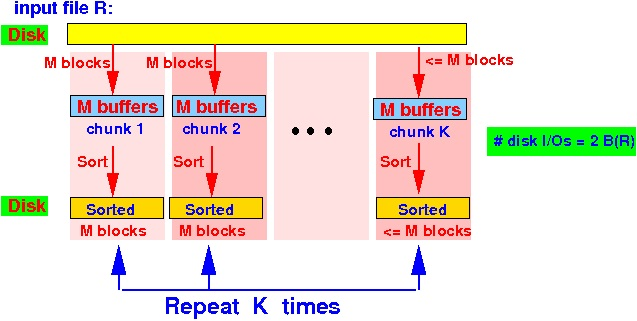
\includegraphics[width=350px]{assets/pass1.jpg}
	\end{figure}

\subsection{Pass 2}
	\begin{enumerate}
		\item We (re)-use the M buffers to merge the first $(Available\ Memory\ Buffer\ -\ 1)$ chucks into a chunk of size $(Available\ Memory\ Buffer)\times(Available\ Memory\ Buffer\ -\ 1)$ blocks
		\item\label{recurse} Iterate over every first element of chunks and pick least value
		\item Output if it is not same as previously picked element
		\item Repeat from Step \ref{recurse} until all the elements in all chunks are evaluated
	\end{enumerate}


\section{Implementation}
The code is implemented in Python as below

\inputminted{python}{../two_pass_sort_based.py}

\subsection{Output}
\inputminted{text}{../output.txt}


\section{Summary}
One pass algorithm can only work if whole block of relation can fit in to main memory otherwise we require more than one pass to determine correct result such as \textbf{Two-Pass Multiway Merge Sort (TPMMS) Algorithm} as implemented here for unary operator - distinct ($\delta$).

For Two pass algorithm we need to fetch all blocks and then write the individually sorted blocks and again we need to read all blocks to perform query operation hence this algorithm can only work if below requirements are satisfied.

\subsection{Requirements of Two Pass}

\begin{itemize}
	\item $number\ of\ chunks\ \leq\ Available\ Memory\ Buffer\ -\ 1$
\end{itemize}

\subsection{File Size Constraint}
\begin{itemize}
	\item $Max\ File\ Size\ \leq\ (Available\ Memory\ Buffer)\times(Available\ Memory\ Buffer\ -\ 1)$
\end{itemize}


\end{document}
